\chapter{Symbology: Single symbol}

\pagestyle{fancy}
\fancyhf{}
\fancyhead[OC]{\leftmark}
\fancyhead[EC]{\rightmark}
%\renewcommand{\footrulewidth}{1pt}
\cfoot{\thepage}

The symbology of a layer is its visual appearance on the map.

Let's change the symbology of the World layer using the \textit{Layers Styling} panel. Either open this panel using menu: View $\rightarrow$ Panels  $\rightarrow$ Layer Styling, or the icon in the top of the \textit{Layers} panel  \begin{tabular}{@{}c@{}}
\includegraphics[width=4ex]{images/layer_styling_panel_icon.png}\end{tabular}. Default location for the \textit{Layers Styling} panel is on the RHS of the window.


\section{Create a landmass and a coastline}

Since we may not always have access to internet - like today - let's learn about single symbol symbology to turn the World layer (with grey area and black border) into a landmass and coast.\\

Within the \emph{Layers Styling} panel follow these steps (and use the screenshots below to help guide you to the correct part):
1. Select layer: uk\\
2. Select Simgle symbol\\
3. In the top white box, highlight the option "Fill"\\
4. Click on Color bar to access the color selector pane\\
5. Select colour for the landmass\\
6. Click blue triange to return to previous pane\\
7. In the top white box, highlight the option "Simple fill"\\
8. Select same colour for stroke colour as landmass (use either "Recent colours" or "Pick colour")\\
9. Expand \textit{Layer Rendering}\\
10. Enable Draw effect\\
11. Click on yellow star (\textit{Customize effects})\\
12. Select \& highlight \textit{Outer Glow} (\emph{select} adds it to the map, \emph{highlight} allows you to change the settings)\\
13. Play about with settings. I chose Spread: 3.2. Blur radius 4.6. Single color: blue. Kept rest as default.\\

\begin{figure}[!h]
	\centering
	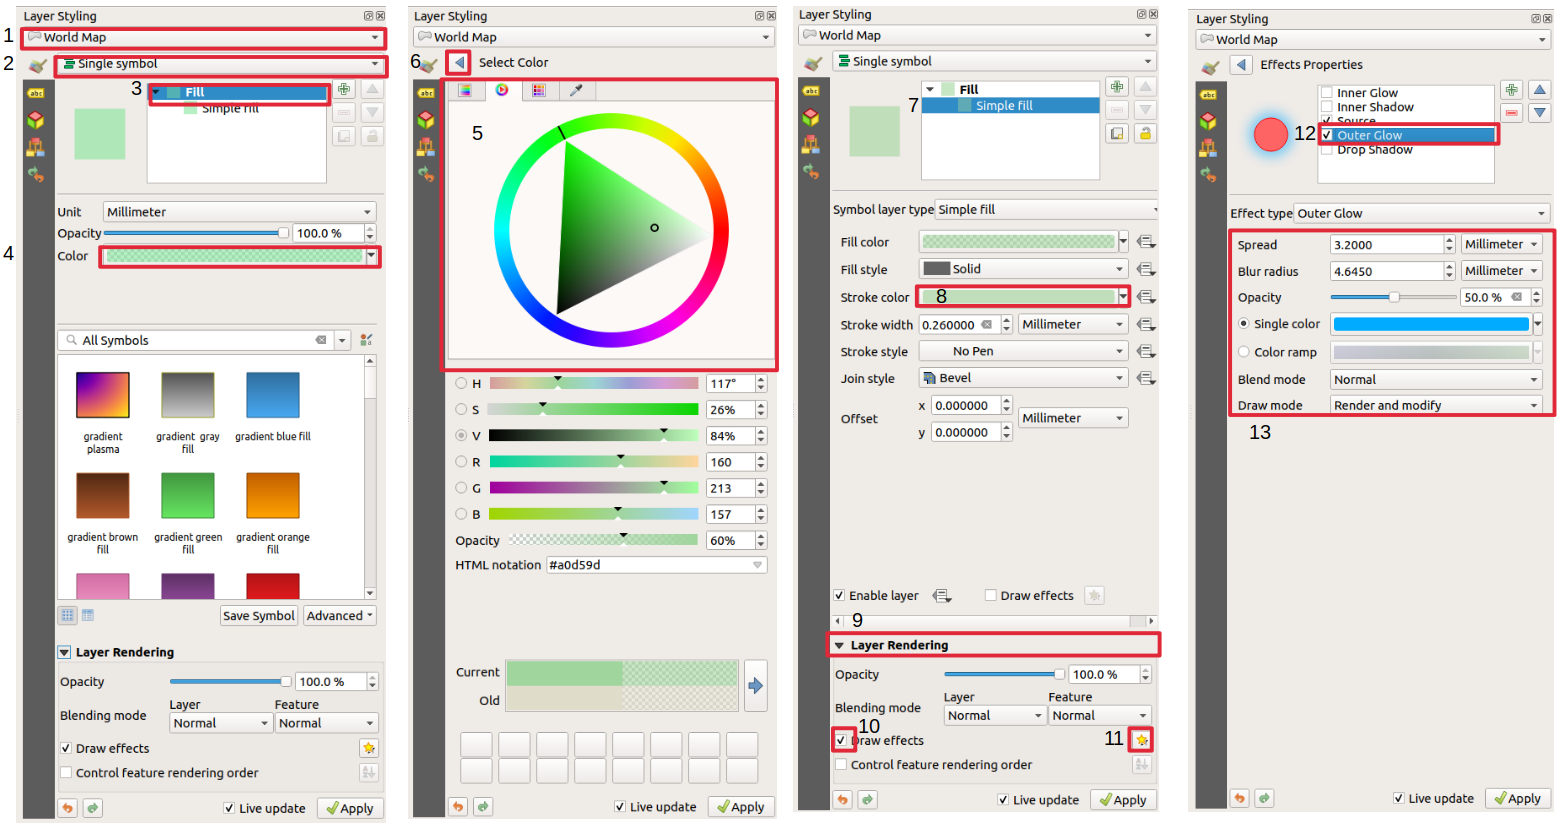
\includegraphics[width=1\textwidth]{images/symb_land_and_sea.png}
	\caption{Settings in Layer Styling to create a landmass and coastal effect}
	\label{ft_fig_firstfig3}
\end{figure}

%\begin{figure}[h!] % "[t!]" placement specifier just for this example
%	\begin{subfigure}{0.28\textwidth}
%		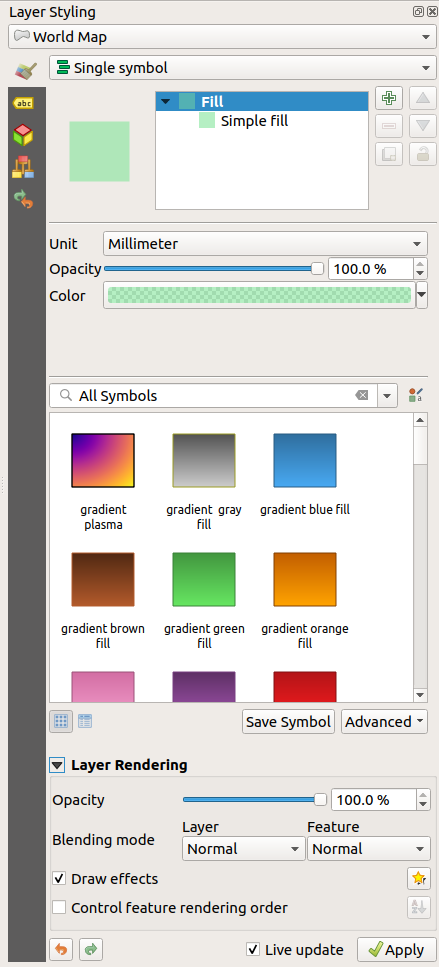
\includegraphics[width=\linewidth]{images/sglsym_stage1.png}
%		\caption{Equal interval} \label{Equal interval}
%	\end{subfigure}\hspace*{\fill}
%	\begin{subfigure}{0.28\textwidth}
%		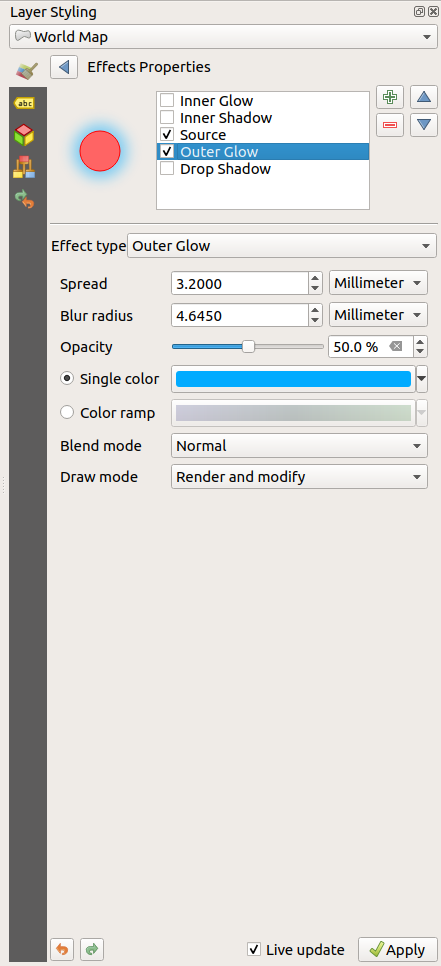
\includegraphics[width=\linewidth]{images/sglsym_stage2.png}
%		\caption{Quantile (Equal count)} \label{Quantile (Equal count)}
%	\end{subfigure}
%\end{figure}

Note1 : Two useful buttons at bottom of Layer Styling panel (Undo \& Redo):            
\begin{tabular}{@{}c@{}}
\includegraphics[width=4ex]{images/styling_redo_undo_icon.png}\end{tabular}.\\

Note 2: Steps \#12 \& \#13 be careful that you have the right option highlighted in the top window before you make changes in the settings below. It is possible to overwrite the \textit{Effect type}.\\


\begin{figure}[!h]
	\centering
	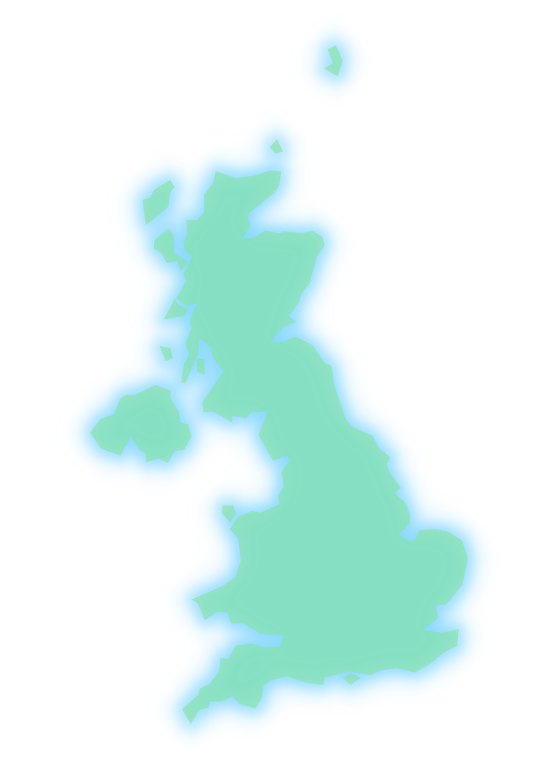
\includegraphics[width=0.5\textwidth]{images/uk_with_coast.png}
	\caption{Using simple symbol to create a landmass and coastal effect}
	\label{ft_fig_firstfig3}
\end{figure}

This uk layer is a shapefile. We will explore more about shapefiles in a couple of chapters.